\section*{Materiale}

Il materiale utilizzato per questa esperienza di laboratorio è il seguente:

\begin{itemize}
    \setlength{\itemsep}{1pt}
	\item{Resistenza ($R$) variabile con un'incertezza nominale dell'$1\,\%$;}
	\item{Osilloscopio: Agilent Technologies in grado di distiguere frequenze di massimo $70\,\si{\mega\hertz}$;}
	\item{AC Power Supply, che è il nostro trasformatore;}
	\item{Multimetro: Agilent Technologies;}
\end{itemize}

L'errore che abbiamo attribuito alle misure prese mediante il multimero e l'oscilloscopio è quello di risoluzione dello strumento, che a seconda del tipo di misura assume un valore differente.

\section*{Circuito}

\begin{wrapfigure}{r}{0.5\textwidth}
    \vspace{-1cm}
    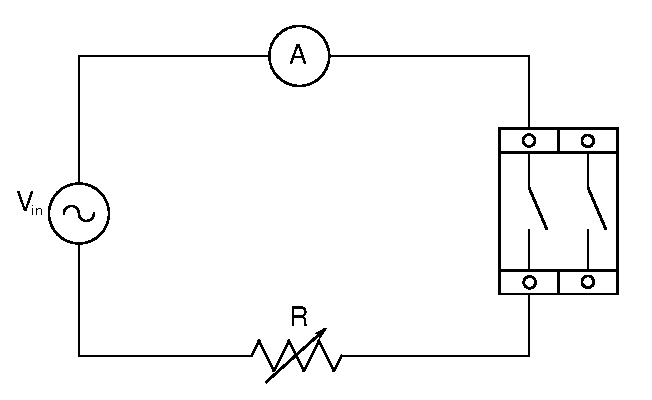
\includegraphics[width=0.48\textwidth]{sc.pdf}
    \caption{Circuito}
    \label{fig:circuito}
    \vspace{-1cm}
\end{wrapfigure}

Ricordiamo che per tutta la durata dell'esperienza la differenza di potenziale utilizzata è stata di $\SI{7.5}{\volt}\,\text{rms}$ ad una frequenza di $\SI{50}{\hertz}$. Inoltre il nostro circuito è alimentato con corrente alternata.
